\documentclass[conference]{IEEEtran}
\IEEEoverridecommandlockouts
% The preceding line is only needed to identify funding in the first footnote. If that is unneeded, please comment it out.
%Template version as of 6/27/2024

\usepackage{cite}
\usepackage{amsmath,amssymb,amsfonts}
\usepackage{algorithmic}
\usepackage{graphicx}
\usepackage{textcomp}
\usepackage{xcolor}
\usepackage{hyperref}
\usepackage{array}
\usepackage{arydshln}
\usepackage{multicol}
\usepackage{wrapfig}
\usepackage{listings}
\newcolumntype{P}[1]{>{\centering\arraybackslash}p{#1}}
\newcolumntype{M}[1]{>{\centering\arraybackslash}m{#1}}


\begin{document}

\title{3D Vehicle Reconstruction via Monocular Camera with Deep Learning Models and Direct Linear Transformation\\
{\footnotesize 2024-2 Robot Vision (M3228.003000)}
}

\author{
    \IEEEauthorblockN{Thomas Putzer}
    \IEEEauthorblockA{\textit{Computer Science and Engineering} \\
        \textit{Seoul National University}\\
        Seoul, South Korea \\
        putzer\_thomas@snu.ac.kr}
    \and
    \IEEEauthorblockN{Weihao Chao}
    \IEEEauthorblockA{\textit{Mechanical Engineering} \\
        \textit{Seoul National University}\\
        Seoul, South Korea \\
        email address or ORCID}
    \and
    \IEEEauthorblockN{Anggraini Ditha}
    \IEEEauthorblockA{\textit{Civil and Environmental Engineering} \\
        \textit{Seoul National University}\\
        Seoul, South Korea \\
        email address or ORCID}
}

\maketitle

\begin{abstract}
    Hello here goes the abstract
\end{abstract}

\section{Introduction}
\begin{center}
    \cite{main-article}
    (Leave this citation for now, otherwise it breaks (if we have 0 citations, and the command at the end))
\end{center}

Bla Bla Bla Bla

\section{3d Pose Estimation}
\setcounter{MaxMatrixCols}{20}

($A = U\Sigma V^{T}$)
\cite{SVD}
In the SVD $Ab = U\Sigma V^{T}b = 0$ implies $V^{T}b = 0$ since $U$ is invertible and has no nontrivial solutions for $Ub = 0$.
Thus $V^{T}b$ must be a vector where only the rows corresponding to zero singular values contribute to the null space.
The columns of $V$ that correspond to zero singular values in $\Sigma$ combined form a basis for the null space of $A$.

\[
    \renewcommand{\arraystretch}{1.5}
    \left[\begin{array}{@{}c:c@{}}
            R                        & t \\ \hdashline
            \begin{array}{@{}ccc@{}}
                0 & 0 & 0
            \end{array} & 1
        \end{array}\right]
\]

$\leq$

\begin{lstlisting}[language=Python, basicstyle=\small, tabsize=4]
#Pseudo code of the matching process
#cars keeps track of all the cars in the scene
#cars_n contains all the cars in the new frame
for old_car in cars:
    c, d = closest_car(cars_n, old_car)
	if d > max_distance:
        #the car left the frame
	    cars.remove(old_car)
	else:
        old.match(c)
        #every car can only be matched once
        cars_n.remove(new_car)

#all remaining not matched new cars
for new_car in cars_n: 
    #a new car has entered the frame 
    cars.append(new_car) 
\end{lstlisting}


\begin{multicols}{2}

    double column text here. .double column text here. . .
    double column text here. . .
    double column text here. . .
    double column text here. . .lkasj fundingasdf

    lsakdfj laks ich icha heise laskdjf lasdffi cich ic ach
    .

\end{multicols}
lkasdjf lakjsd flkajsdl fkjasdl fjasldj flaskdjf laskdjf laksjdfl kajsdflkajsdlfjasldkfjalsdkjflaskjdf laskdjf lasjkdfl aksjdflkasjd flaskjdf lkasdjf lkasjdf laksjdfl akjsdlfj asldkfj alsdjkf lasdjf laskdjf laskdjf laksdjfl aksdjfl askdjl askjf l

\begin{equation}
    FOV = 2 \cdot \arctan\left(\frac{s_w}{2f}\right),
    r = n \cdot \tan\left(\frac{FOV}{2}\right)
\end{equation}

\begin{figure}
    \centering
    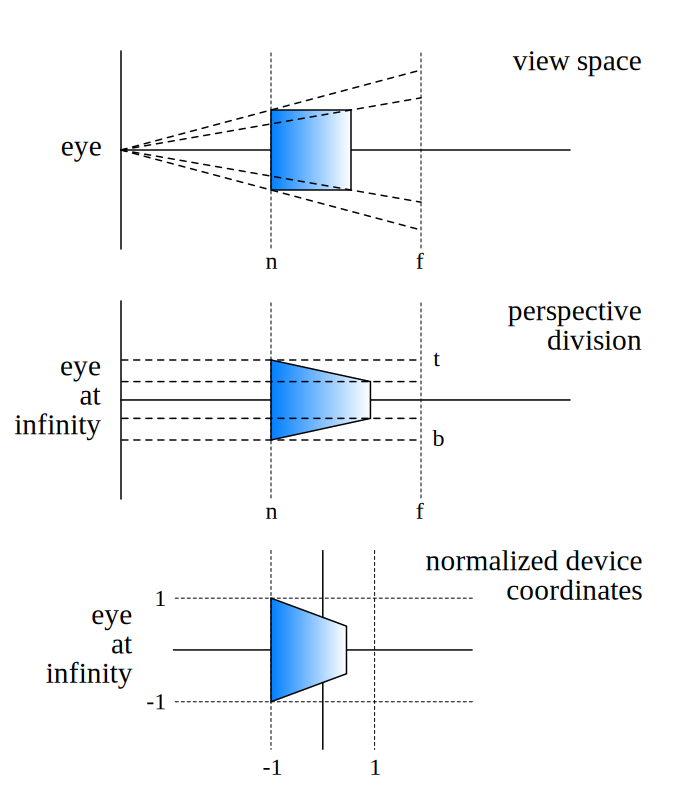
\includegraphics[width=0.8\columnwidth]{./images/view_coordinates_to_ndc.png}
    \caption{Perspective projection from view space to NDC}
    \label{img:view_to_ndc}
\end{figure}

\begin{figure}
    \centering
    \includegraphics[width=0.7\columnwidth]{./images/wireframes.png}
    \caption{Different car wireframes used. From left to right Ford Explorer, Volvo V60, Nissan Altima.}
    \label{img:wireframes}
\end{figure}

double column text here. .double column text here. . .
double column text here. . .
double column text here. . .
double column text here. . .lkasj fundingasdf
double column text here. .double column text here. . .
double column text here. . .
double column text here. . .
double column text here. . .lkasj fundingasdf
double column text here. .double column text here. . .
double column text here. . .
double column text here. . .
double column text here. . .lkasj fundingasdf

\begin{wrapfigure}{L}{0.5\columnwidth}
    \centering
    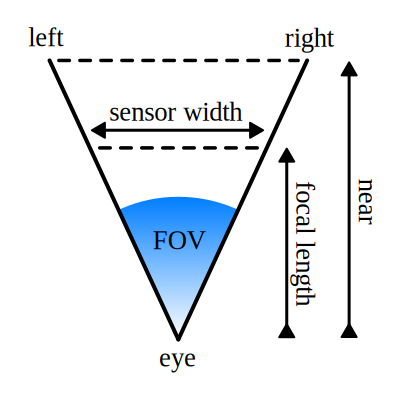
\includegraphics[width=0.45\columnwidth]{./images/focal_lenght_and_field_of_view.png}
    \caption{The sensor width and the focal length are used to calculate the camera's field of view.}
    \label{img:fov}
\end{wrapfigure}

double column text here. .double column text here. . .
double column text here. . .
double column text here. . .
double column text here. . .lkasj fundingasdf
double column text here. .double column text here. . .
double column text here. . .
double column text here. . .
double column text here. . .lkasj fundingasdf

Matrix representation of the standard projection onto the z = 1 plane.
\begin{equation}
    \begin{bmatrix}
        1 & 0 & 0 & 0 \\
        0 & 1 & 0 & 0 \\
        0 & 0 & 1 & 0 \\
        0 & 0 & 1 & 0
    \end{bmatrix}
    \begin{bmatrix}
        x \\
        y \\
        z \\
        1
    \end{bmatrix}
    =
    \begin{bmatrix}
        x \\
        y \\
        z \\
        z
    \end{bmatrix}
    \overset{\text{div z}}{\equiv}
    \begin{bmatrix}
        \frac{x}{z} \\
        \frac{y}{z} \\
        1           \\
    \end{bmatrix}
\end{equation}

The API projection Matrix

\twocolumn[
    \begin{equation} \label{eqn:API_matrix}
        M_{P} = M_{P''} M_{P'} =
        \begin{bmatrix}
            \frac{2}{r - l} & 0               & 0               & \frac{-(r + l)}{r - l} \\
            0               & \frac{2}{t - b} & 0               & \frac{-(t + b)}{t - b} \\
            0               & 0               & \frac{2}{f - n} & \frac{-(f + n)}{f - n} \\
            0               & 0               & 0               & 1
        \end{bmatrix}
        \begin{bmatrix}
            n & 0 & 0     & 0   \\
            0 & n & 0     & 0   \\
            0 & 0 & n + f & -nf \\
            0 & 0 & 1     & 0
        \end{bmatrix}
        =
        \begin{bmatrix}
            c_1 & 0   & 0   & 0   \\
            0   & c_2 & 0   & 0   \\
            0   & 0   & c_3 & c_4 \\
            0   & 0   & 1   & 0
        \end{bmatrix}
    \end{equation}
    \begin{equation} \label{eqn:DLT}
        \begin{bmatrix}
            -c_1 x_1 & -c_1 y_1 & -c_1 z_1 & -c_1   & 0        & 0        & 0        & 0      & x_1 x_{1}' & y_1 x_{1}' & z_1 x_{1}' & x_{1}' \\
            0        & 0        & 0        & 0      & -c_2 x_1 & -c_2 y_1 & -c_2 z_1 & -c_2   & x_1 y_{1}' & y_1 y_{1}' & z_1 y_{1}' & y_{1}' \\
            \vdots   & \vdots   & \vdots   & \vdots & \vdots   & \vdots   & \vdots   & \vdots & \vdots     & \vdots     & \vdots     & \vdots \\
            -c_1 x_n & -c_1 y_n & -c_1 z_n & -c_1   & 0        & 0        & 0        & 0      & x_n x_{n}' & y_n x_{n}' & z_n x_{n}' & x_{n}' \\
            0        & 0        & 0        & 0      & -c_2 x_n & -c_2 y_n & -c_2 z_n & -c_2   & x_n y_{n}' & y_n y_{n}' & z_n y_{n}' & y_{n}' \\
        \end{bmatrix}
        \begin{bmatrix}
            a      \\
            b      \\
            \vdots \\
            k      \\
            l
        \end{bmatrix}
        =
        \begin{bmatrix}
            0      \\
            0      \\
            \vdots \\
            0      \\
            0
        \end{bmatrix}
    \end{equation}
]

To get the screen-space position of a vertex, we multiply it by its Modelview Matrix and API Projection Matrix before doing the projective division.
We have all the parameters except the Model Matrix. $p' = M_{API} M_{Modelview} p$

\begin{equation*}
    \begin{bmatrix}
        x' \\
        y' \\
    \end{bmatrix}
    \overset{\text{div w}}{\equiv}
    \begin{bmatrix}
        c_1 & 0   & 0   & 0   \\
        0   & c_2 & 0   & 0   \\
        0   & 0   & c_3 & c_4 \\
        0   & 0   & 1   & 0
    \end{bmatrix}
    \begin{bmatrix}
        a & b & c & d \\
        e & f & g & h \\
        i & j & k & l \\
        0 & 0 & 0 & 1
    \end{bmatrix}
    \begin{bmatrix}
        x \\
        y \\
        z \\
        1
    \end{bmatrix}
\end{equation*}

If we multiply that out, we get for $x'$ and $y'$:

\begin{gather*}
    x' = \frac{c_1 a x + c_1 b y + c_1 c z + c_1 d}{ix + jy + kz + l} \\
    y' = \frac{c_2 e x + c_2 f y + c_2 g z + c_2 h}{ix + jy + kz + l}
\end{gather*}

We can multiply by the denuminator and solve for 0. Since this holds for every pair of points $(p_{1} , p_{1}'), (p_{2} , p_{2}'), ..., (p_{n}, p_{n}')$ that we track we can create the following system of equation:
\ref{eqn:DLT}


\bibliographystyle{./IEEEtran.bst}
\bibliography{./robot_vision}

\end{document}
